\section{Control Plots}
\label{sec:GBJ1:Uncorr}
This section presents the selected data compared to the reconstructed PYTHIA sample, to check that the PYTHIA sample approximately agrees with data.
This is necessary if the MC is to be used for systematic studies and unfolding.


Figure \ref{UncorrIncl_dy} shows the \Incl{} distribution for (a)~$70<\ptb{}<90$ GeV, (b)~$90<\ptb{}<120$ GeV and (c)~$180<\ptb{}<210$ GeV slices. 
The MC and data shape agree, with differences of less than 10\%.
Figure \ref{Uncorr_Pt3_dy} shows the \ptDist{} distribution, where $\pt{}^{veto}$ is the \pt{} of the highest jet in the rapidity region bounded by the dijet system,  for two different slices in \dy{} and \ptb{}. 
The shape of the PYTHIA prediction has adequate agreement with data in both regions, with fluctuations of about 20\%.
The main differences are at higher \pt{} where the statistical uncertainty is higher.
Figure \ref{Uncorr_GF} shows slices of the gap fraction against \dy{} and \ptb{}.
As a function of \dy{}, PYTHIA describes the data well, only deviating by $\approx10\%$ at higher \dy{}.
As a function of \ptb{}, PYTHIA describes the data very well for $\ptb{}<250$ GeV, after that the gap fraction for PYTHIA is $\approx10\%$ high.
The three figures demonstrate reasonable agreement between the data and the reconstructed PYTHIA sample. 
This was true of other control plots and the forward/backward dijet selection.
Overall, there is confidence that the PYTHIA sample can be used for systematic studies and for correcting detector effects. 
These control plots are also published in \cite{ref:ATLASGap}.

\begin{figure}
\centering
        \begin{subfigure}[b]{0.5\textwidth}
                \centering
                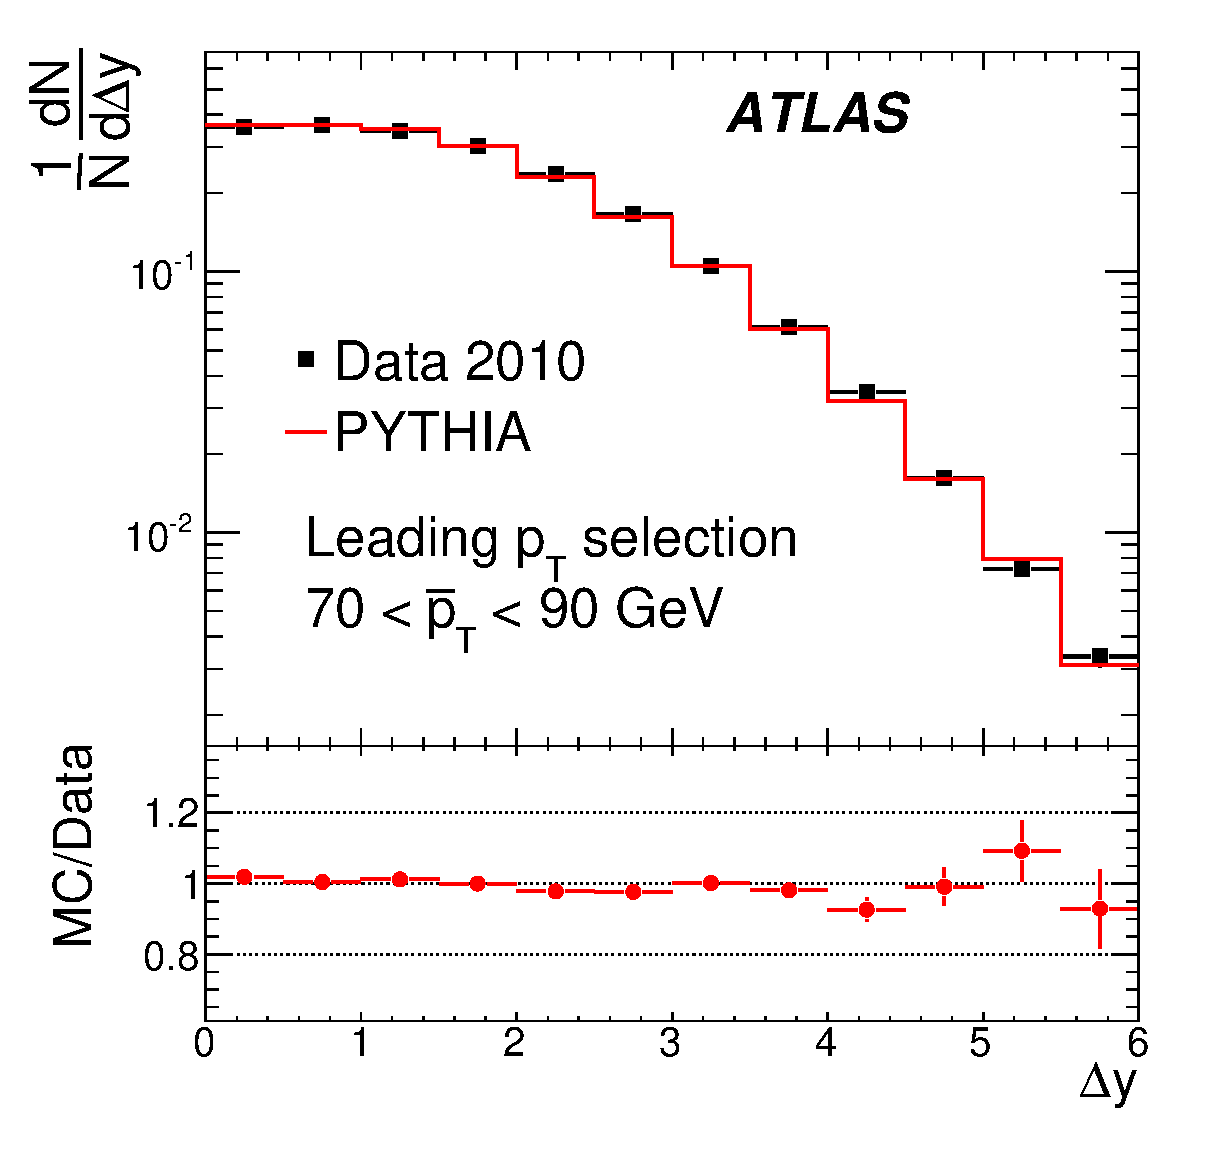
\includegraphics[width=\textwidth]{figures/GBJ1/UncorrectedData/Inclusive_selA_Ave_pT_70_90_Norm.eps}
        \end{subfigure}%
        \begin{subfigure}[b]{0.5\textwidth}
                \centering
                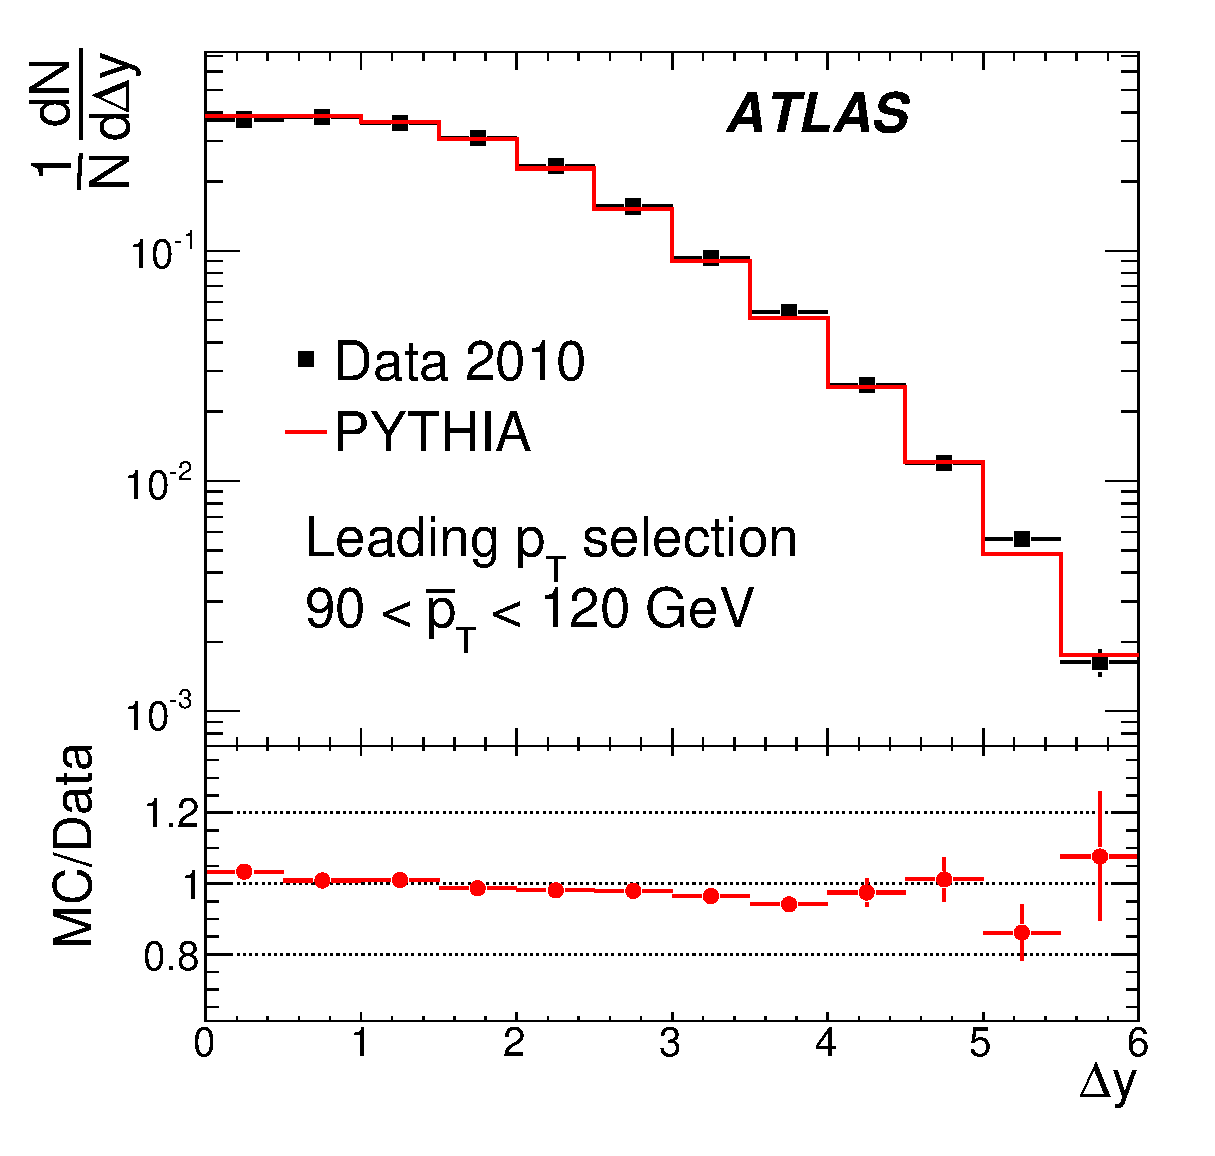
\includegraphics[width=\textwidth]{figures/GBJ1/UncorrectedData/Inclusive_selA_Ave_pT_90_120_Norm.eps}
        \end{subfigure}%

        \begin{subfigure}[b]{0.5\textwidth}
                \centering
                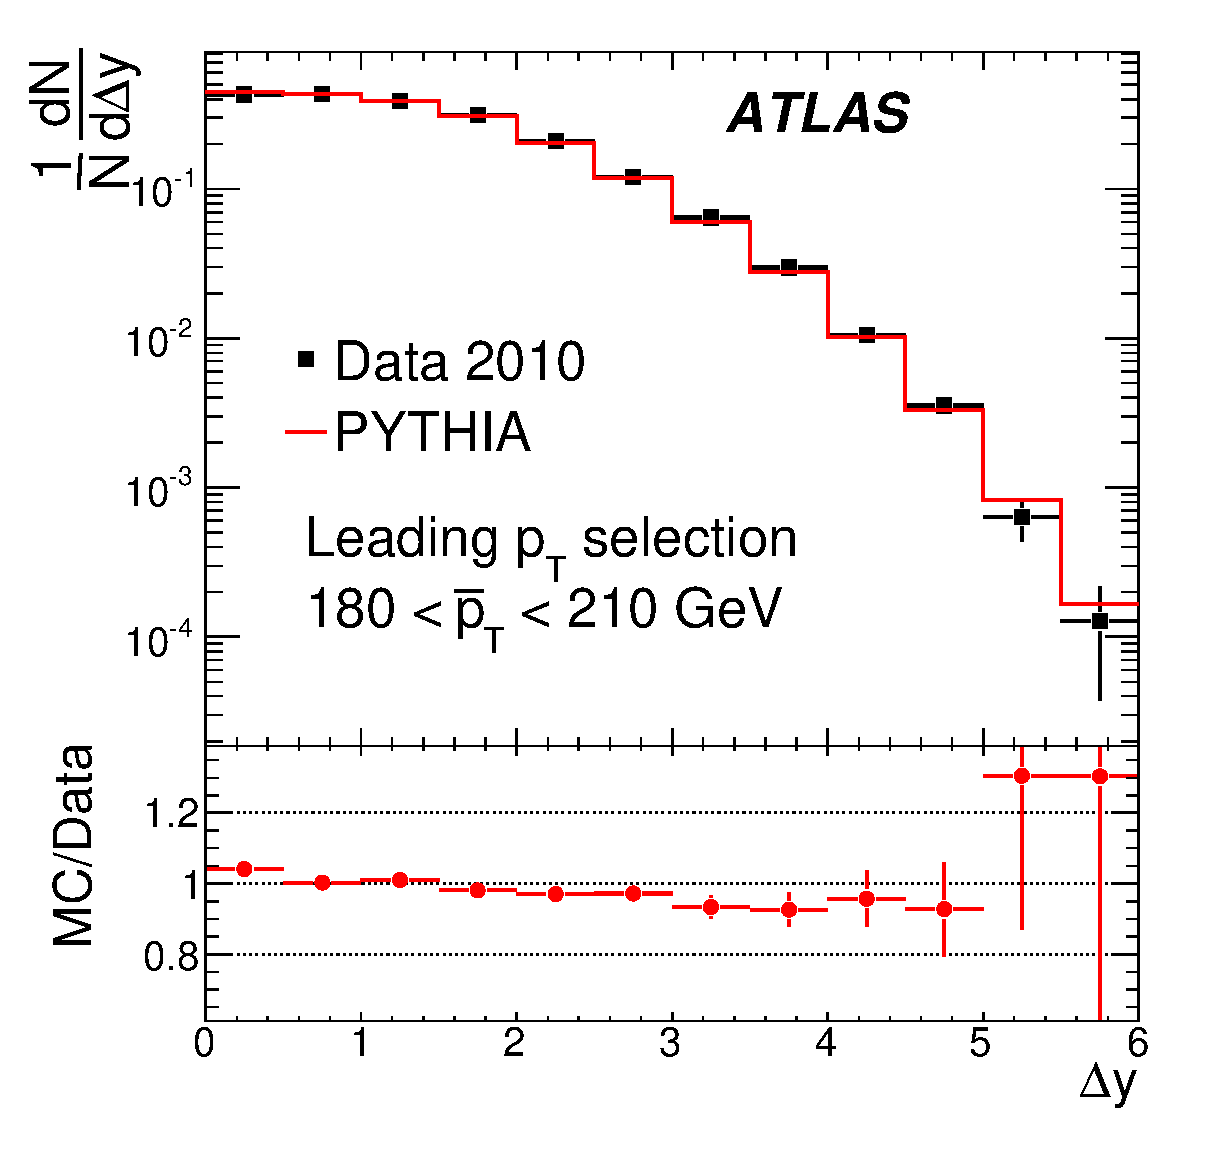
\includegraphics[width=\textwidth]{figures/GBJ1/UncorrectedData/Inclusive_selA_Ave_pT_180_210_Norm.eps}
        \end{subfigure}%

\caption[Comparison of the inclusive distribution versus \dy{} between the data and the reconstructed PYTHIA sample for the leading \pt{} dijet selection]{
Fraction of events for each \dy{} bin for the 2010 uncorrected data and the reconstructed PYTHIA sample for leading \pt{} dijet selection. 
Shown are (a) $70<\ptb{}<90$~GeV, (b) $90<\ptb{}<120$~GeV and (c) $210<\ptb{}<240$~GeV slices.
\label{UncorrIncl_dy}}
\end{figure}

\begin{figure}
\centering
        \begin{subfigure}[b]{0.5\textwidth}
                \centering
                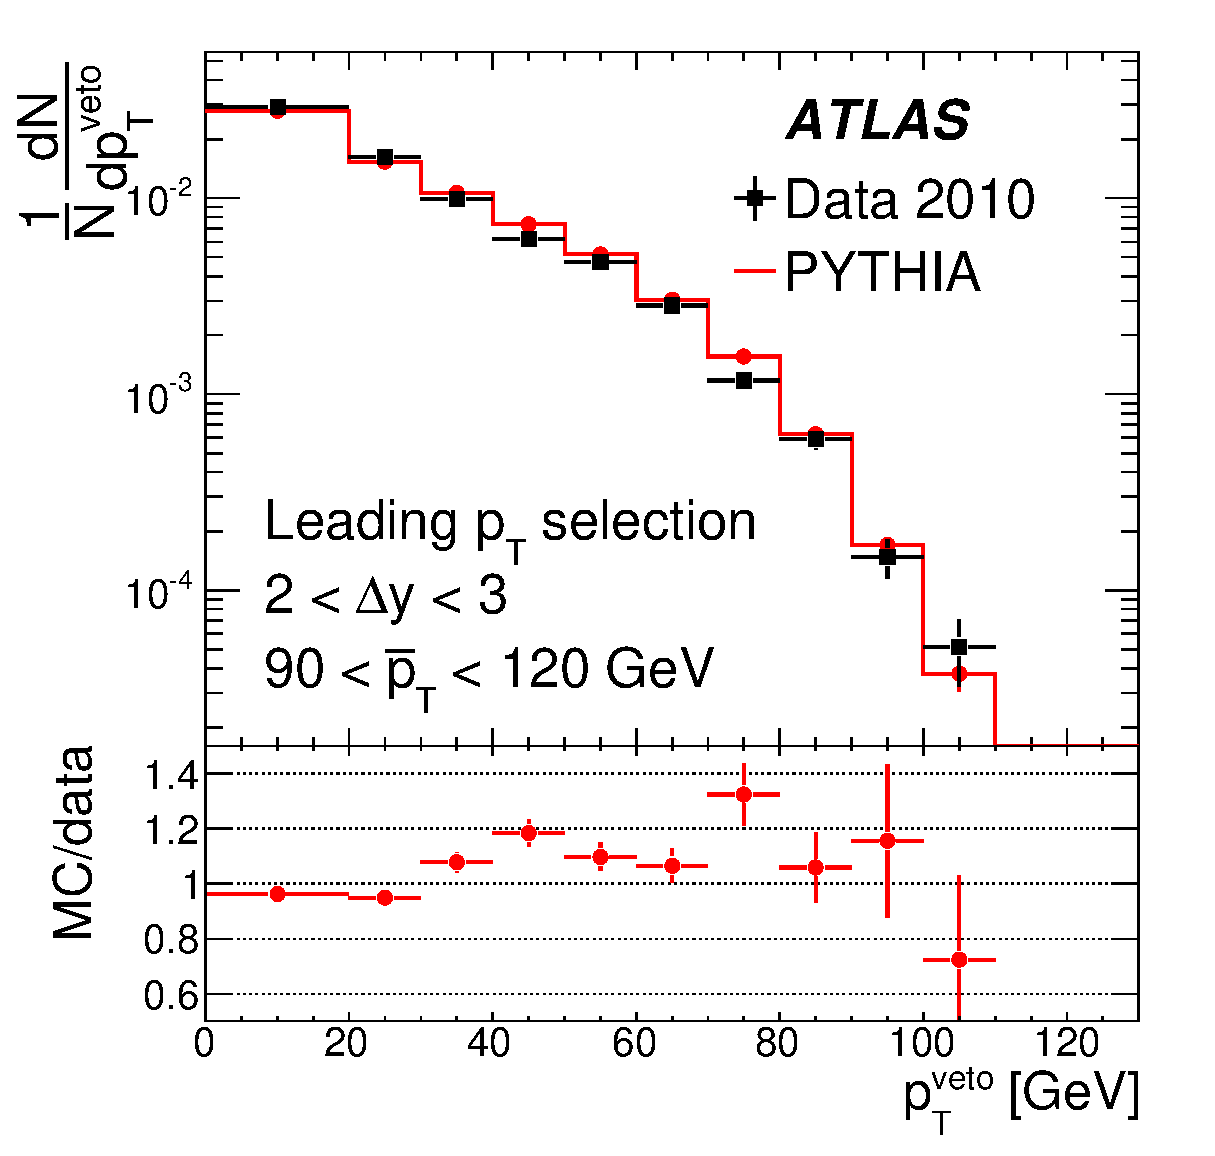
\includegraphics[width=\textwidth]{figures/GBJ1/UncorrectedData/Pt3_dY_2_3_pt_90_120_PYTHIA.eps}
        \end{subfigure}%
        \begin{subfigure}[b]{0.5\textwidth}
                \centering
                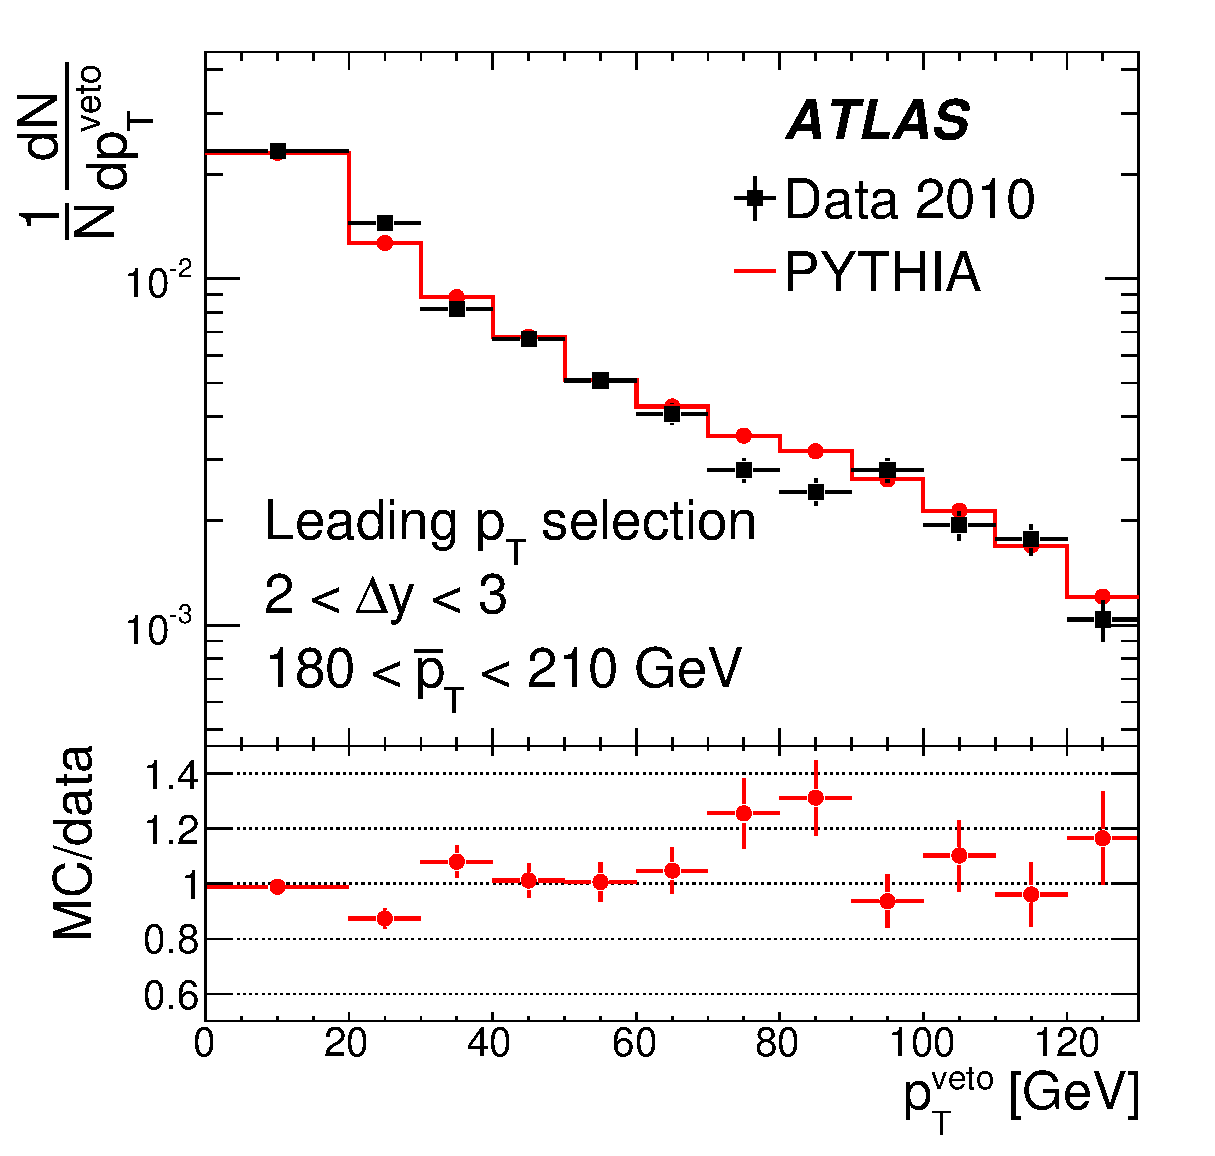
\includegraphics[width=\textwidth]{figures/GBJ1/UncorrectedData/Pt3_dY_2_3_pt_180_210_PYTHIA.eps}
        \end{subfigure}%
\caption[Comparison of $p_T^{veto}$ distribution between the data and the reconstructed PYTHIA sample ]{
Faction of events for each $p_T^{veto}$ bin for the 2010 uncorrected data and the reconstructed PYTHIA sample, where $\pt{}^{veto}$ is the \pt{} of the highest jet in the rapidity region bounded by the dijet. 
Shown are (a) $90<\ptb{}<120$~GeV and $2 < \dy{} <3$, and (b) $90<\ptb{}<120$~GeV and $2 < \dy{} <3$ slices.
\label{Uncorr_Pt3_dy}}
\end{figure}

\begin{figure}
\centering
        \begin{subfigure}[b]{0.5\textwidth}
                \centering
                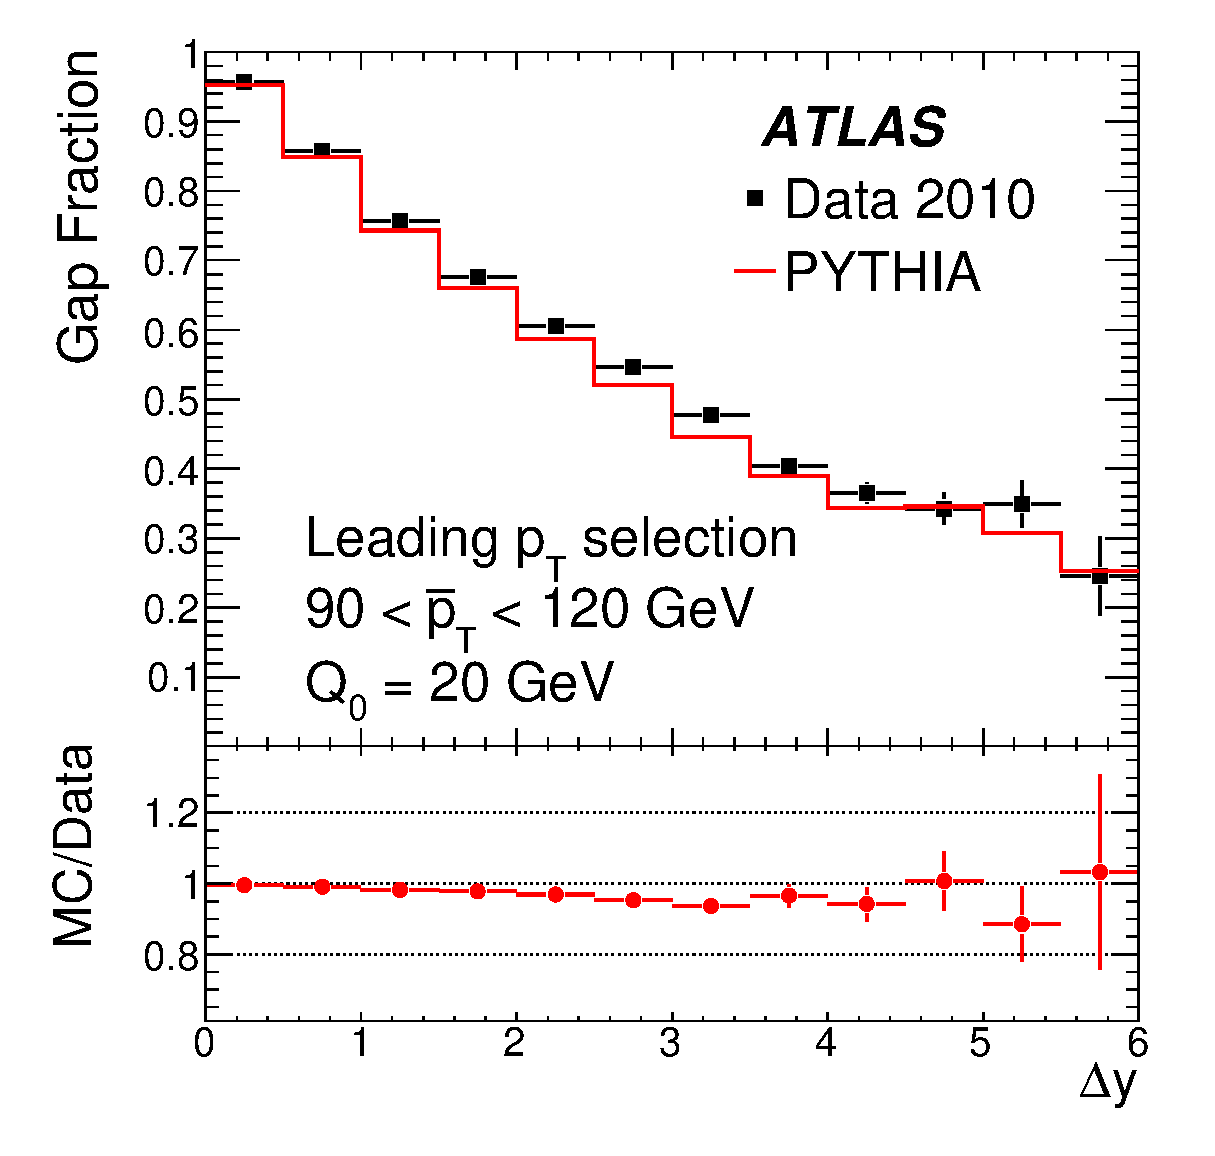
\includegraphics[width=\textwidth]{figures/GBJ1/UncorrectedData/RatioGF_selA_Ave_pT_90_120.eps}
        \end{subfigure}%
        \begin{subfigure}[b]{0.5\textwidth}
                \centering
                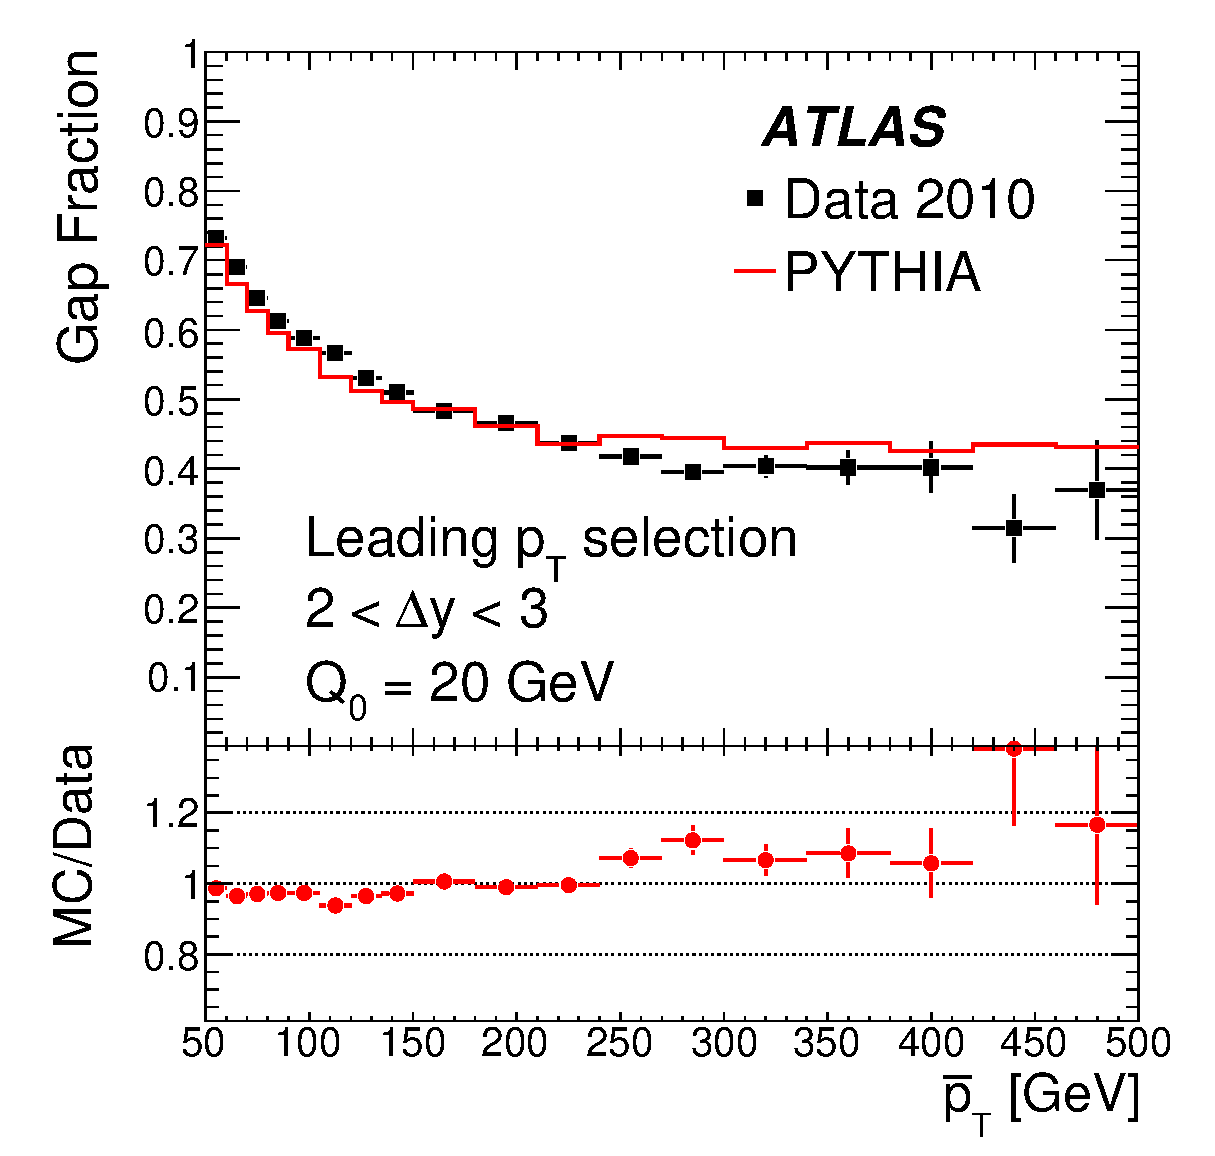
\includegraphics[width=\textwidth]{figures/GBJ1/UncorrectedData/RatioGF_selA_DeltaY_2_3.eps}
        \end{subfigure}%
\caption[Comparison of gap fraction versus \dy{} and \ptb{} between the data and the reconstructed PYTHIA sample for leading \pt{} dijet selection]{
Gap fraction against (a) \dy{} for the $90<\ptb{}<120$~GeV slice and (b) \ptb{} for the $2 < \dy{} <3$ slice, for the 2010 uncorrected data and the PYTHIA sample for the leading \pt{} dijet selection.
\label{Uncorr_GF}}
\end{figure}


